\documentclass[10.5pt,a4paper]{article}

% -------------------- Page Layout & Geometry --------------------
\usepackage[a4paper,margin=1.7cm,top=1.6cm,bottom=1.6cm]{geometry}
\usepackage{setspace}
\setstretch{1.06}
\setlength{\parindent}{0pt}
\setlength{\parskip}{0.4em}
\setlength{\emergencystretch}{2.5em}

% -------------------- Typography --------------------
\usepackage{iftex}
\ifPDFTeX
  \usepackage[T1]{fontenc}
  \usepackage[utf8]{inputenc}
  \usepackage{lmodern}
\else
  \usepackage{fontspec}
  \setmainfont{Noto Sans}[Scale=0.98, BoldFont=* Bold, ItalicFont=* Italic]
  \setsansfont{Noto Sans}[Scale=0.98]
  \setmonofont{Noto Sans Mono}[Scale=0.92]
\fi

% -------------------- Core Packages --------------------
\usepackage{graphicx}
\graphicspath{{./}{figures/}}
\usepackage{booktabs}
\usepackage{tabularx}
\usepackage{array}
\usepackage{enumitem}
\usepackage{xcolor}
\usepackage{hyperref}
\usepackage{caption}
\usepackage{subcaption}
\usepackage{amsmath}
\usepackage{amssymb}
\usepackage{tikz}
\usetikzlibrary{arrows.meta,positioning,shapes.geometric,calc}
\usepackage{fancyhdr}
\usepackage{titlesec}
\usepackage{microtype}

% Float control: prevent premature page breaks
\renewcommand{\topfraction}{0.90}
\renewcommand{\bottomfraction}{0.85}
\renewcommand{\textfraction}{0.10}
\renewcommand{\floatpagefraction}{0.85}
\setlength{\floatsep}{6pt plus 2pt minus 2pt}
\setlength{\textfloatsep}{8pt plus 2pt minus 2pt}
\setlength{\intextsep}{6pt plus 2pt minus 2pt}

% -------------------- Minimalist High-Contrast Colors --------------------
\definecolor{TextDark}{HTML}{111827}
\definecolor{GrayDark}{HTML}{374151}
\definecolor{GrayLight}{HTML}{F3F4F6}
\definecolor{BorderGray}{HTML}{D1D5DB}

% -------------------- Hyperlinks (Clean & High-Contrast) --------------------
\hypersetup{
  colorlinks=true,
  linkcolor=black,
  urlcolor=black,
  citecolor=black,
  pdftitle={MyStorage Assignment Report - Nguyen Anh Phi},
  pdfauthor={Nguyen Anh Phi}
}

% -------------------- Header & Footer --------------------
\pagestyle{fancy}
\setlength{\headheight}{18pt}
\fancyhf{}
\lhead{\textcolor{GrayDark}{\footnotesize MyStorage Assignment Report}}
\rhead{\textcolor{GrayDark}{\footnotesize Product Engineering Intern (AI-Native)}}
\cfoot{\textcolor{GrayDark}{\footnotesize Page \thepage}}
\renewcommand{\headrulewidth}{0.4pt}
\renewcommand{\headrule}{\hbox to\headwidth{\color{BorderGray}\leaders\hrule height \headrulewidth\hfill}}

% -------------------- Section Formatting --------------------
\titleformat{\section}
  {\large\bfseries\color{TextDark}}
  {\thesection.}{0.45em}{}
\titlespacing*{\section}{0pt}{8pt}{3pt}

\titleformat{\subsection}
  {\normalsize\bfseries\color{TextDark}}
  {\thesubsection}{0.45em}{}
\titlespacing*{\subsection}{0pt}{6pt}{2pt}

\setlist[itemize]{leftmargin=1.3em,topsep=2pt,itemsep=1.5pt,parsep=0pt}
\setlist[enumerate]{leftmargin=1.3em,topsep=2pt,itemsep=1.5pt,parsep=0pt}

\begin{document}

% ============================================================
% Title & Candidate Metadata Block
% ============================================================
\begin{center}
  {\LARGE\bfseries\color{TextDark} MYSTORAGE ASSIGNMENT REPORT}\par
  \vspace{0.25em}
  {\normalsize\bfseries\color{TextDark} Product Engineering Intern (AI-Native) --- STOW 2.0 Audit \& Prototype}\par
\end{center}

\vspace{0.1em}

\begin{tabularx}{\textwidth}{>{\bfseries}p{3.8cm} >{\raggedright\arraybackslash}X}
\toprule
Candidate Name: & Nguyen Anh Phi \\
Email / Phone: & \href{mailto:phina1011@gmail.com}{phina1011@gmail.com} $\;\mid\;$ (+84) 352 689 716 \\
GitHub Repository: & \url{https://github.com/AnhPhiNe/mystorage-ai-native} \\
Live Demo Prototype: & \url{https://mystorage-ai-native.streamlit.app} \\
Hours Spent: & \textasciitilde 5 hours (Audit: 1.5h $\mid$ Prototype \& LangGraph: 2.5h $\mid$ Benchmark \& Report: 1h) \\
\bottomrule
\end{tabularx}

\vspace{0.3em}

\section{Executive Summary \& Audit Findings on stow.mystorage.vn}

By testing \href{https://stow.mystorage.vn}{\texttt{stow.mystorage.vn}} from the perspective of an actual prospective customer and benchmarking responses against the official website and canonical \href{https://mystorage.vn/llms.txt}{\texttt{/llms.txt}} knowledge base, I identified three high-impact issues directly affecting \textbf{Revenue} and \textbf{Customer Trust}.

\subsection*{Finding 1: Scoping Error \& Policy Hallucination in Insurance Compensation (Severity: CRITICAL)}

\textbf{What Happened:}
\begin{enumerate}
  \item When asked about compensation for a 3 m\textsuperscript{3} unit under the Basic tier, STOW asserted: \textit{``mức bồi thường tối đa là 10.000.000 VNĐ ạ''}. STOW conflated the \textbf{theoretical global plan cap} with the \textbf{actual per-unit compensation limit} derived from its volume (3 m\textsuperscript{3} $\times$ 500,000 VND = \textbf{1,500,000 VND}).
  \item When asked about paid protection tiers (tested in both Vietnamese \textit{``Bạc, Vàng, Bạch kim''} and English \textit{``Silver, Gold, Platinum''}), STOW flatly denied their existence: \textit{``Dạ hiện tại MyStorage \textbf{không} có các gói tên Bạc, Vàng hay Bạch kim ạ''}, despite these tiers being documented in \texttt{/llms.txt} and the booking portal.
\end{enumerate}

\textbf{Steps to Reproduce:} Query 1: \textit{``Kho 3m\textasciicircum 3 dùng gói Basic được bồi thường tối đa bao nhiêu ?''} $\rightarrow$ Query 2: \textit{``MyStorage có gói bảo hiểm Bạc, Vàng, Bạch kim không''}.

\textbf{Why it Matters:} Causes direct loss of high-margin upsell revenue (50k--200k/month). Furthermore, it introduces acute legal liability and customer disputes when a damaged 3 m\textsuperscript{3} unit contractually receives only 1.5M VND rather than the promised 10M VND.

\textbf{Proposed Fix:} Decouple arithmetic from the LLM by implementing a deterministic Python tool \texttt{calculate\_insurance(cbm, plan)}.

\begin{figure}[htbp]
  \centering
  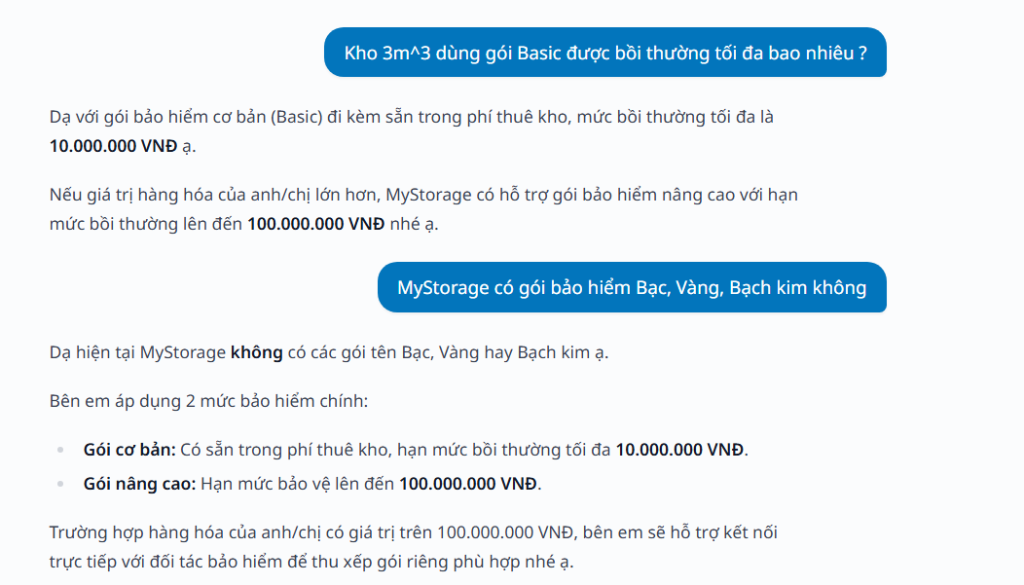
\includegraphics[width=0.72\textwidth]{insurance_chat.png}
  \caption{Finding 1 Illustration: STOW reports the 10M VND cap for a 3 m\textsuperscript{3} unit and explicitly denies paid protection tiers.}
  \label{fig:insurance-finding}
\end{figure}

\subsection*{Finding 2: Hallucination of Language-Specific Branch Hotlines \& Mobile Numbers (Severity: HIGH)}

\textbf{What Happened:} When urgently requesting contact channels, STOW extrapolated numeric patterns from the single official landline (\texttt{028 7770 0117}) and invented fictional branch lines and an unauthorized mobile number:
Vietnamese Support (\texttt{028 7771 0118}), Korean Support (\texttt{028 7771 0119}), Japanese Support (\texttt{028 7771 0120}), Emergency Access (\texttt{0868 208 079}).

\textbf{Steps to Reproduce:} Query: \textit{``tui muốn liên hệ gấp với bên stow thì nên dùng đường dây nào vậy hãy liệt kê các đường dây nóng mà cậu có đi''}.

\textbf{Why it Matters:} During critical operations (e.g., customers locked out of 24/7 facilities at night), calling disconnected numbers leads to operational failure, acute frustration, and severe brand damage.

\textbf{Proposed Fix:} Introduce a dedicated \texttt{get\_contact\_info()} tool returning strictly \texttt{028 7770 0117} and \texttt{hello@mystorage.vn}, coupled with negative prompt constraints preventing fictional extensions.

\begin{figure}[htbp]
  \centering
  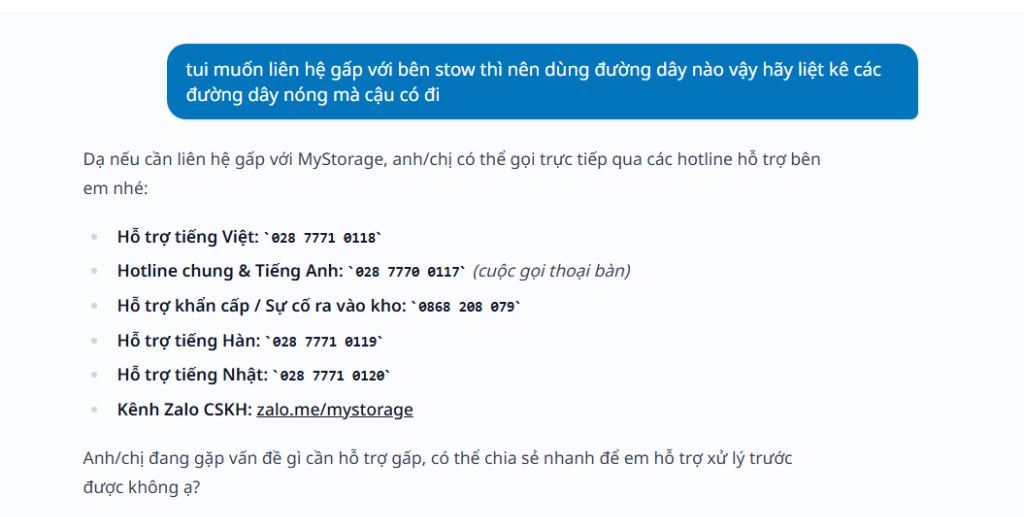
\includegraphics[width=0.72\textwidth]{hotline_hallucination.png}
  \caption{Finding 2 Illustration: STOW invents fictional language branch extensions and an unauthorized emergency mobile number.}
  \label{fig:hotline-finding}
\end{figure}

\subsection*{Finding 3: Missing Direct Booking Call-To-Action (CTA) Leading to Funnel Drop-off (Severity: MEDIUM)}

\textbf{What Happened:} After resolving unit sizing or pricing inquiries, STOW concludes passively (\textit{``Do you have any further questions?''}) without presenting an actionable booking link directing users to the official booking flow (\url{https://booking.mystorage.vn/en/book?step=service}).

\textbf{Why it Matters:} Introduces unnecessary friction into the sales pipeline. High-intent customers must navigate back to the main website to book, resulting in conversion drop-off.

\textbf{Proposed Fix:} Introduce proactive booking CTA triggers into the agent's workflow, generating direct booking links upon resolving sizing or service intent.

\section{Working Prototype \& Architecture (STOW 2.0)}

To solve these root causes under an \textbf{AI-Native} approach, I developed the \textbf{STOW 2.0} prototype using Python, \textbf{LangGraph / ReAct Agent}, \textbf{Streamlit UI}, and \textbf{DeepInfra} (\texttt{deepseek-ai/DeepSeek-V4.1-Flash}).

\subsection*{Architecture Overview}

\begin{figure}[htbp]
\centering
\resizebox{0.92\textwidth}{!}{%
\begin{tikzpicture}[
  node distance=12mm and 11mm,
  box/.style={draw=BorderGray, thick, rounded corners=2mm, minimum height=9mm, minimum width=32mm, align=center, fill=white},
  agent/.style={box, draw=TextDark, fill=GrayLight, minimum width=44mm},
  tool/.style={box, draw=TextDark, fill=GrayLight, minimum width=44mm, minimum height=14mm},
  arrow/.style={-{Latex[length=2.5mm]}, thick, draw=GrayDark}
]
  \node[box] (customer) {Customer};
  \node[box, right=of customer] (ui) {Streamlit UI};
  \node[agent, right=of ui] (agent) {LangGraph ReAct Agent};

  \node[tool, below left=16mm and -1mm of agent] (kb) {Tool 1: KB Search\\\footnotesize Grounded facts from \texttt{llms.txt}};
  \node[tool, below=16mm of agent] (calc) {Tool 2: Insurance Calc\\\footnotesize Deterministic Python math};
  \node[tool, below right=16mm and -1mm of agent] (contact) {Tool 3: Contact Info\\\footnotesize Canonical hotline 028 7770 0117};

  \draw[arrow] (customer) -- (ui);
  \draw[arrow] (ui) -- (agent);
  \draw[arrow] (agent) -- (kb);
  \draw[arrow] (agent) -- (calc);
  \draw[arrow] (agent) -- (contact);
\end{tikzpicture}%
}
\caption{STOW 2.0 Architecture: Decoupling probabilistic reasoning (LLM) from deterministic arithmetic and verified facts (Python Tools).}
\label{fig:architecture}
\end{figure}

\subsection*{Empirical Prototype Verification \& Tool Tracing}

The interactive Streamlit prototype demonstrates how the ReAct agent executes deterministic tools to eliminate hallucinations in real time:

\begin{figure}[htbp]
  \centering
  \begin{subfigure}[t]{0.48\textwidth}
    \centering
    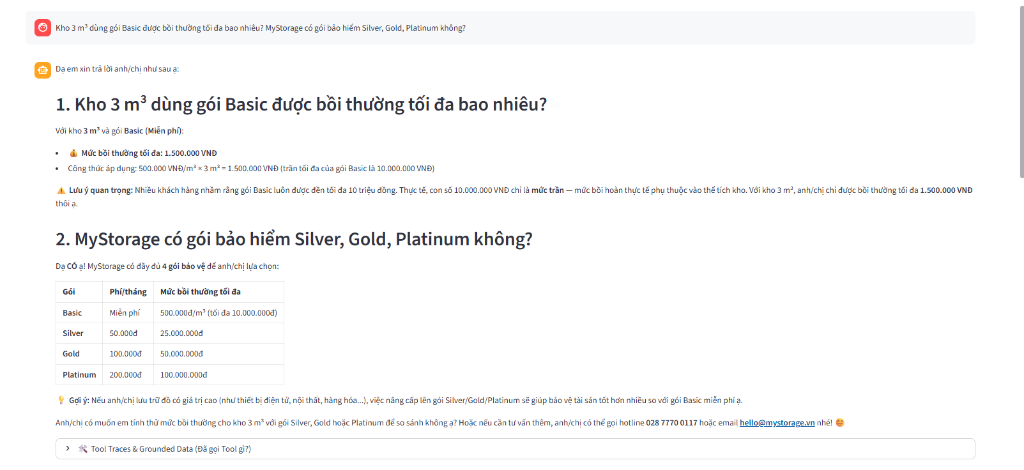
\includegraphics[width=\linewidth]{prototype_insurance.png}
    \caption{\textbf{Resolution of Finding 1:} Executes \texttt{calculate\_insurance} for exact 1.5M VND arithmetic and displays all 4 tiers.}
    \label{fig:proto-insurance}
  \end{subfigure}
  \hfill
  \begin{subfigure}[t]{0.48\textwidth}
    \centering
    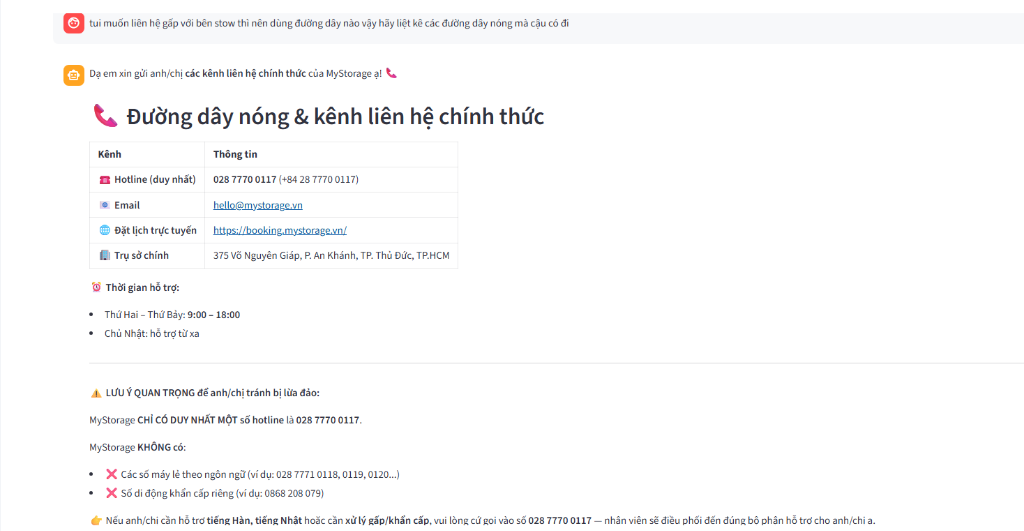
\includegraphics[width=\linewidth]{prototype_hotline.png}
    \caption{\textbf{Resolution of Finding 2:} Invokes \texttt{get\_contact\_info} returning only 028 7770 0117, warning against fictional branch lines.}
    \label{fig:proto-hotline}
  \end{subfigure}
  
  \vspace{0.4em}
  
  \begin{subfigure}[t]{0.48\textwidth}
    \centering
    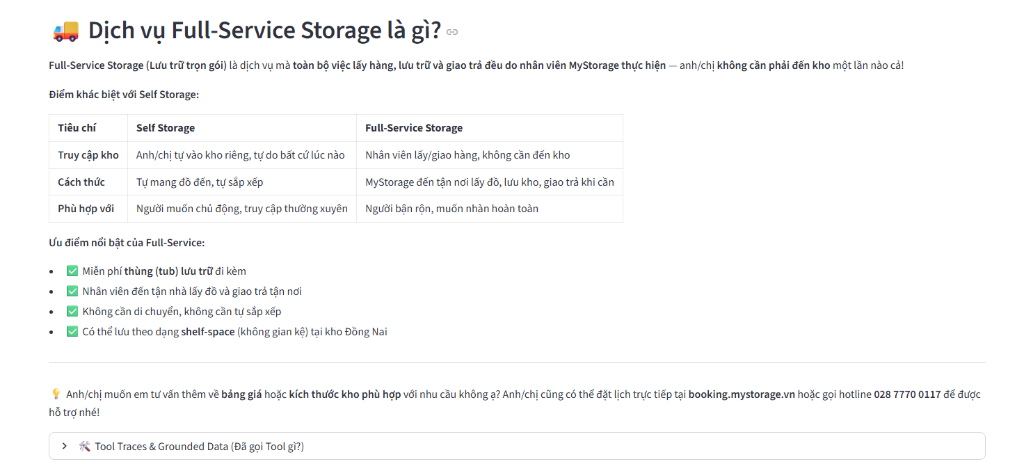
\includegraphics[width=\linewidth]{prototype_booking_cta.png}
    \caption{\textbf{Resolution of Finding 3:} Explains service differences and surfaces an immediate, direct booking Call-to-Action link.}
    \label{fig:proto-cta}
  \end{subfigure}
  \hfill
  \begin{subfigure}[t]{0.48\textwidth}
    \centering
    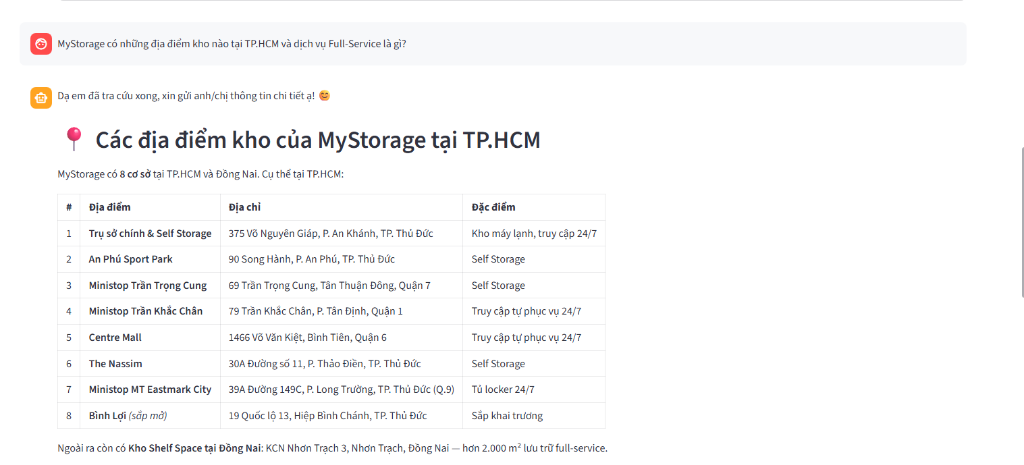
\includegraphics[width=\linewidth]{prototype_locations.png}
    \caption{\textbf{Grounded Knowledge Retrieval:} Invokes \texttt{search\_mystorage\_kb} to accurately list all verified facilities across HCMC.}
    \label{fig:proto-locations}
  \end{subfigure}
  \caption{STOW 2.0 Live Prototype Verification: UI traces showing tool calling, deterministic outputs, and proactive conversion CTAs.}
  \label{fig:prototype-verification}
\end{figure}

\subsection*{Automated Benchmark Evaluation}

Executing the automated benchmark suite via \texttt{eval.py} demonstrated total correctness:

\begin{table}[htbp]
\centering
\small
\renewcommand{\arraystretch}{1.25}
\begin{tabularx}{\textwidth}{>{\bfseries}p{3.2cm} >{\raggedright\arraybackslash}X >{\raggedright\arraybackslash}X >{\centering\arraybackslash}p{1.6cm}}
\toprule
Evaluation Metric & Baseline (Original STOW) & STOW 2.0 (Grounded Agent) & Result \\
\midrule
Paid Protection Tiers & Denies Silver/Gold/Platinum exist & Accurately lists all 4 tiers: Basic, Silver, Gold, Platinum & \textbf{PASS} \\
3 m\textsuperscript{3} Unit Payout & Falsely quotes 10M VND plan cap & Accurately calculates \textbf{1,500,000 VND} (3 $\times$ 500k) & \textbf{PASS} \\
Contact Hotlines & Hallucinates 1900..., 028 7771 0118... & Exclusively provides \textbf{028 7770 0117} & \textbf{PASS} \\
\bottomrule
\end{tabularx}
\caption{Automated Benchmark Comparison: Baseline vs. STOW 2.0 (100\% pass rate across 6/6 test assertions).}
\end{table}

\section{What Claude Code Produced That I Rejected or Rewrote, and Why}

\begin{quote}
\small\itshape
``What 'AI-native' means here: Claude Code is our default way of building. You read every line the model produces and you can defend it in review. If you can't explain it, it doesn't ship.''
\end{quote}

\begin{itemize}
  \item \textbf{What Was Rejected:} When prompted to address the insurance calculation discrepancy, the AI assistant initially generated an extended \textbf{System Prompt Engineering} solution---attempting to instruct the LLM to perform inline arithmetic within its generation chain.
  \item \textbf{Why It Was Rejected:} Large Language Models are fundamentally probabilistic token predictors, not arithmetic engines. Relying strictly on prompt instructions for dynamic pricing, volume-based insurance math, and contact invariants inevitably fails under conversational pressure or complex customer prompts. In a commercial pipeline, mathematical inaccuracies create unacceptable operational and legal risks.
  \item \textbf{What Was Rewritten:} I rejected prompt-based arithmetic and engineered a \textbf{Deterministic Python Tool} (\texttt{calculate\_insurance}) hooked into a LangGraph ReAct agent. The LLM handles natural language understanding and parameter extraction, while Python code guarantees 100\% arithmetic accuracy.
\end{itemize}

\section{What I Would Do With Two More Hours}

Given two additional hours, I would implement:
\begin{enumerate}
  \item \textbf{Contextual Deeplink Generator:} When a customer agrees on a 3 m\textsuperscript{3} unit in District 7, the agent dynamically generates a pre-populated booking link (\url{https://booking.mystorage.vn/en/book?size=3&facility=d7}) to maximize conversion.
  \item \textbf{Session Memory Persistence:} Integrate LangGraph Checkpointer with Redis/SQLite to persist customer context across sessions and browser tabs.
  \item \textbf{Synthetic Edge-Case Evaluation Suite:} Expand \texttt{eval.py} to run automated regression tests against 50+ adversarial queries, including decimal volumes and coupon edge cases.
\end{enumerate}

\section{Short Note for Application Endpoint (\textless{} 300 words)}

\begin{quote}
\small\itshape
``What's the last thing you built with an AI coding tool, and what did you have to fix yourself?''
\end{quote}

\textbf{Project Experience:} The last system I built with an AI coding tool is a \textbf{Multi-Cohort RAG Chatbot} for the HCMUE Student Handbook, designed to handle complex tabular queries, multi-intent decomposition, and cross-cohort policy comparisons.

My primary engineering tool was \textbf{Claude Code}. While accelerating development, the agent exhibited two recurring failure modes:
\begin{enumerate}
  \item \textbf{Over-engineering \& Context Drift:} Despite defining a strict \texttt{Spec.md} upfront, Claude Code frequently drifted toward bloated architectures, especially after context compaction cycles when earlier constraints were pruned. I had to actively supervise the session, pushing back in code reviews to maintain lean modularity.
  \item \textbf{Brittle Heuristics Over Generalization:} When building the query routing module, Claude Code took naive shortcuts. Rather than evaluating holistic semantic intent, it generated rigid rule-based classification---hardcoding keywords like \textit{``ph\`ong''} (room/department) directly to an \texttt{Office} category, misrouting queries that merely referenced a physical room or unrelated intent.
\end{enumerate}

\textbf{What I fixed myself:} I rejected Claude Code's brittle heuristic logic. Instead, I re-architected the router to use structured semantic classification (enforced via Pydantic schemas) coupled with targeted few-shot intent grounding. I also instituted synthetic edge-case tests to verify that ambiguous phrasing was classified accurately.

This experience reinforced that AI coding assistants naturally optimize for localized quick-fixes; human engineering judgment is essential to enforce modularity, scalability, and robust semantic reasoning.

\end{document}
